The tool that allows us to easily manage bibliography is called BiBTeX. In particular, we are using a \emph{package} called \verb|natbib| that gives us some extra features.
Using it has two distinct moments: Adding an entry to our bibliography, and citing.

\subsection{Creating a bibiliography}
A bibliography file has a \verb|.bib| extension, and each entry has a very specific format.
Let's start with creating the file \verb|bibliography.bib|, so our working directory looks like this:
\begin{verbatim}
Example
├── bibliography.bib
└── example.tex
\end{verbatim}

Each entry has a source, whether \verb|article|, \verb|book|, \verb|misc| or many more and has the following format:
\begin{lstlisting}
@article{ GerberLeahR2005, %Unique identifier
  author    = {Gerber, Leah R and Beger, Maria and McCarthy, Michael A and Possingham, Hugh P},
  title     = {A theory for optimal monitoring of marine reserves},
  issn      = {1461-023X},
  journal   = {Ecology letters},
  pages     = {829--837},
  volume    = {8},
  publisher = {Blackwell Science Ltd},
  number    = {8},
  year      = {2005},
  edition   = {Editor, Ransom Myers Manuscript received 15 March 2005 First decision made 21 April 2005 Manuscript accepted 6 May 2005},
},
\end{lstlisting}

It's worth highlighting that the basic format is essentially \verb|@article{ID,...}|, with each entry being separated by commas.
BiBTeX will handle ``et al'' and other conventions as long as you stick to the following format for the author:
\begin{lstlisting}
author = {LastName1, FirstName1 and LastName2, FirstName2 and...},
\end{lstlisting}

The good side is that you rarely, if ever, need to type it out yourself.
When you find an article through UCL's library, JAMA, Science Direct and many other resources, there will be an option to \textbf{export citation to BiBTeX}.
Simply copy the contents to your bibliography file and you're ready to cite!
\begin{figure}[h]
  \centering
  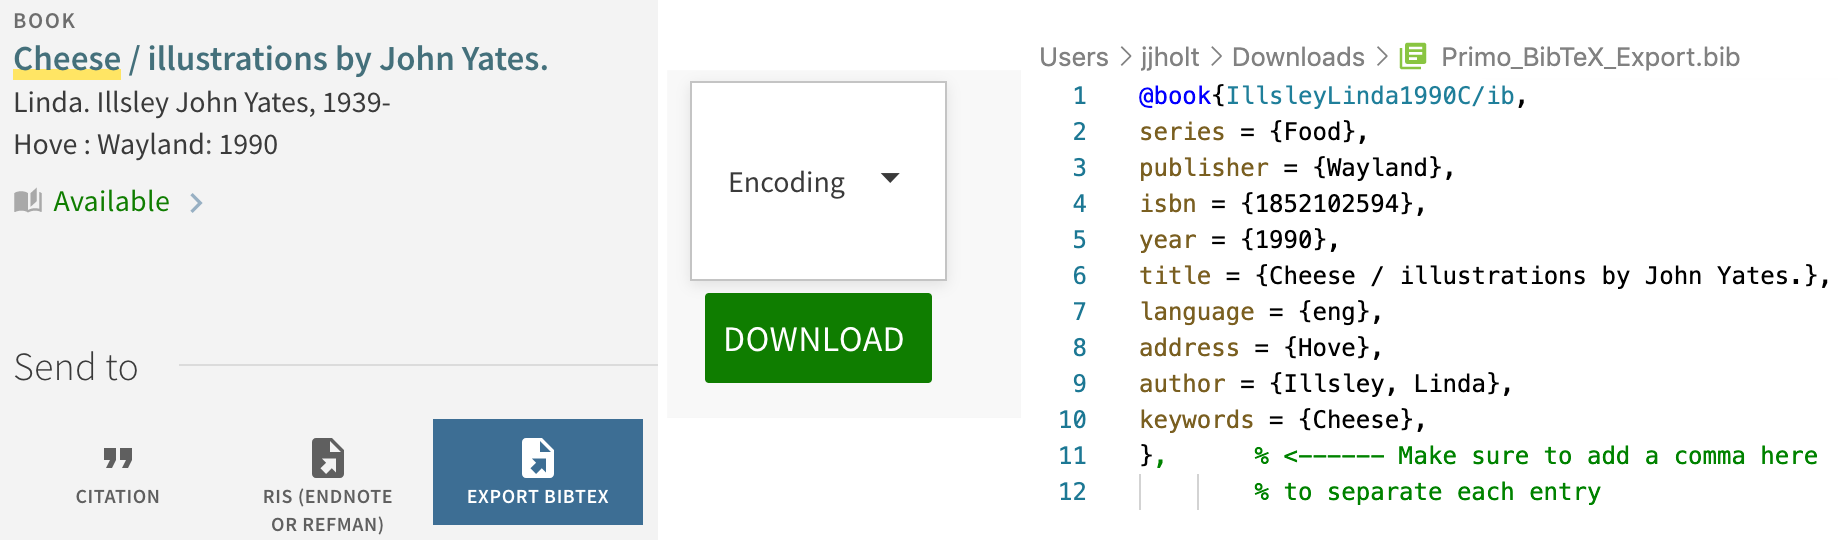
\includegraphics[width=\textwidth]{figures/ucl-lib.png}
  \caption{Getting a BiBTeX file from UCL's Library. From here, just paste to your \texttt{.bib} file.}
  \label{fig:ucl-lib}
\end{figure}

\subsection{Manually adding a bibliography entry}
While in a \verb|.bib| file, you can easily create a scaffold for a bibliography entry.
Simply type \verb|@| and press \verb|Ctrl+space| to see the suggestions.
Generally this is only used for citing random websites, for which we use the \verb|@misc| option.
The scaffold will include all the basic requirements to generate a good bibiliography entry.
\begin{figure}[h]
  \centering
    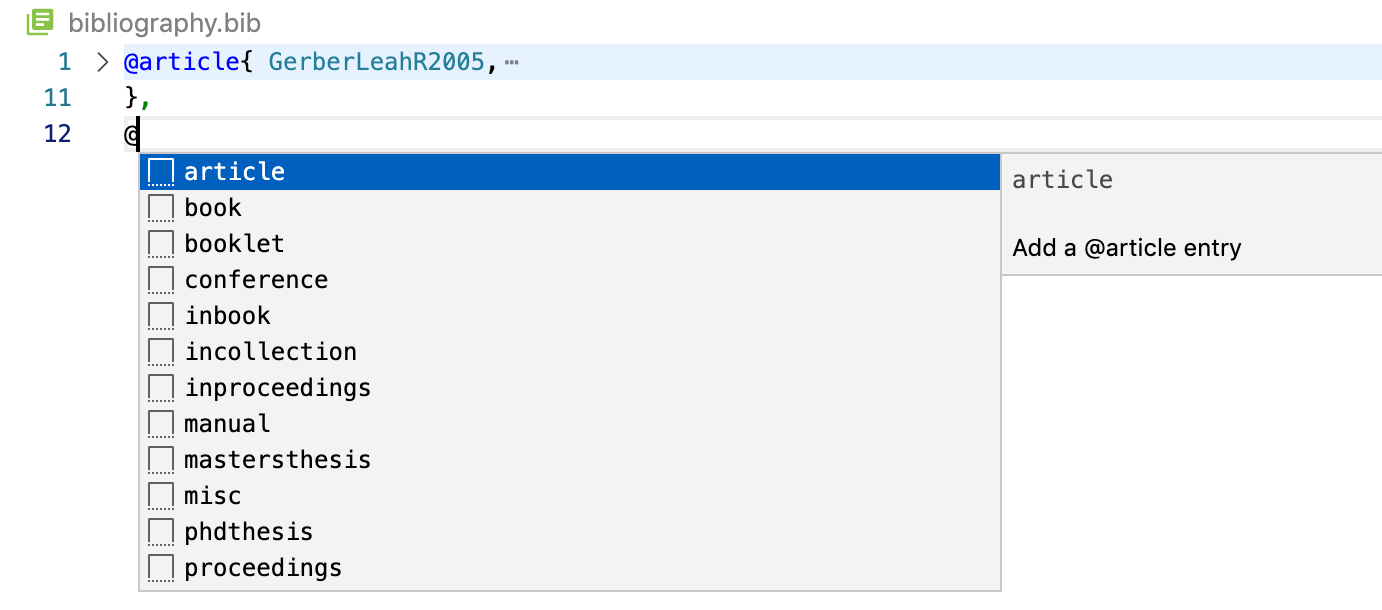
\includegraphics[width=\textwidth]{figures/bib-entry.png}
  \caption{Autocompleting a bibliography entry in a \texttt{.bib} file.}
  \label{fig:bib-entry}
\end{figure}

\subsection{Citations}
Now we just need to let our document know where to find our bibliography file, which we had called \verb|bibliography.bib| and we can use \verb|\cite{}| (or its variants) to do in-text citations.
Every cited entry automatically gets added to a Reference section at the end of the document.
If you want to include any non-cited entry, use \verb|\nocite{id}|; and to include all entries: \verb|\nocite{*}|.
\lstinputlisting[language=tex, caption={example.tex}]{"Example/example.tex"}

Giving us the following output:
\begin{figure}[h]
  \centering
    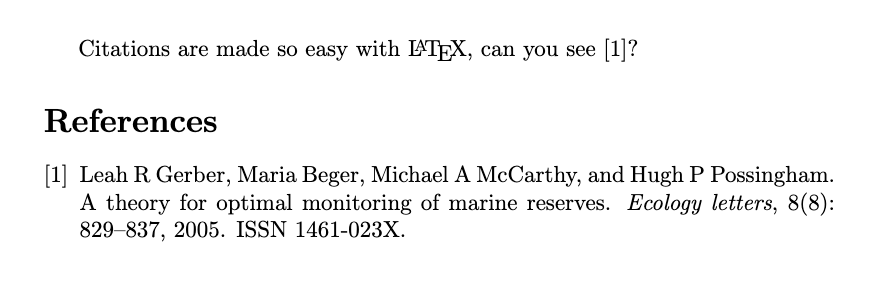
\includegraphics[]{figures/references.png}
  \label{fig:references}
\end{figure}

The options in \verb|\usepackage[square,numbers]{natbib}| are what determine that in-text citations is \textbf{[1]}.
Alternatively if you prefer \textbf{(Gerber et al, 2005)}, use \verb|\usepackage[round]{natbib}|, and \verb|\citep{}| (see code below).
It is also possible to do narrative style citations, such as ``In their work, Gerber et al (2005) describe\dots''. This is achieved with \verb|\cite{}| with this same setting.

\begin{lstlisting}
\usepackage[round]{natbib}
...
\citep{GerberLeahR2005}
...
In their work, \cite{GerberLeahR2005} describe...
\end{lstlisting}

The \verb|natbib| package gives us the \verb|\bibliographystyle{unsrtnat}| command, which determines the style of the references.
There are other styles, as well as more information on \verb|natbib| on \href{https://ftp.eq.uc.pt/software/TeX/macros/latex/contrib/natbib/natnotes.pdf}{this} link. 

\paragraph{Note:}
When citing you may want to include a tilde (\verb|~|) between the last word and \verb|\cite{}|. This guarantees that the citation and the word are on the same line. Like so: \verb|Tomorrow is a day~\cite{GerberLeahR2005}|.

A really important feature of VSCode is Intellisense, these automatic suggestions the editor finds depending on context.
In the case of bibliography, it looks in the \verb|.bib| file we indicate in the preamble, as you can see in Figure \ref{fig:intellisense}.
If you are not getting suggestions, try activating Intellisense by pressing \verb|ctrl+space|.
It also works with various other tags. Try typing \texttt{\textbackslash}, then pressing \verb|ctrl+space| to see the enourmous list.
\begin{figure}[h]
  \centering
  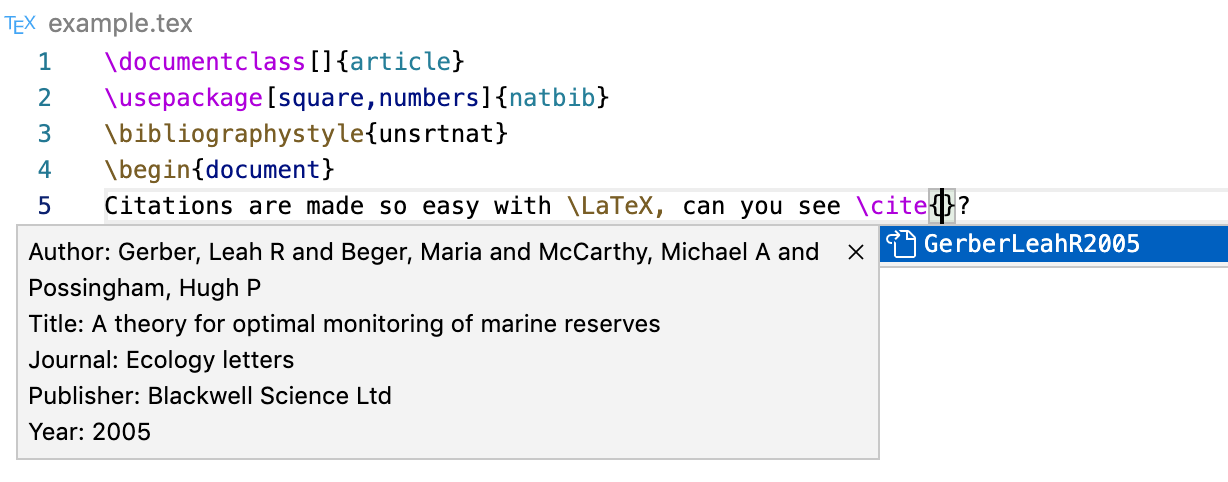
\includegraphics[width=0.8\textwidth]{figures/intellisense.png}
  \caption{Autocomplete from our bibliography file.}
  \label{fig:intellisense}
\end{figure}

Automatically generating the number for figures and tables, and easy cross-referencing are a key feature of \LaTeX.
This means we can refer to a bibliography entry or a figure by its unique id, move it around and it will correctly choose its number.
Before we get into adding all that it is a great idea to take a detour and discuss organisation.